%!TEX program = xelatex
\documentclass[aspectratio=169,11pt]{beamer}

\usetheme{Madrid}
\usecolortheme{default}
\setbeamertemplate{navigation symbols}{}
\setbeamertemplate{caption}[numbered]

\usepackage{fontspec}
% Một họ font duy nhất cho toàn bộ deck: sạch, đồng nhất và dễ đọc khi trình chiếu.
\setsansfont{TeX Gyre Heros}
\setmainfont{TeX Gyre Heros}
\setmonofont{TeX Gyre Heros}
\usepackage{amsmath,amssymb,booktabs,tabularx,tikz,graphicx}
\usetikzlibrary{arrows.meta,positioning,shapes.geometric}
\graphicspath{{figures/}}

\definecolor{accentblue}{RGB}{22,58,105}
\definecolor{accentteal}{RGB}{20,122,112}
\definecolor{accentorange}{RGB}{232,116,28}
\definecolor{softblue}{RGB}{238,246,255}
\definecolor{ink}{RGB}{25,33,45}
\definecolor{navy}{RGB}{25,33,45}
\definecolor{blue}{RGB}{22,58,105}
\definecolor{gold}{RGB}{232,116,28}
\definecolor{muted}{RGB}{25,33,45}
\definecolor{green}{RGB}{20,122,112}
\definecolor{red}{RGB}{190,55,40}
\definecolor{purple}{RGB}{22,58,105}

\setbeamercolor{normal text}{fg=ink,bg=white}
\setbeamercolor{structure}{fg=accentblue}
\setbeamercolor{frametitle}{fg=white,bg=accentblue}
\setbeamercolor{title}{fg=white}
\setbeamercolor{subtitle}{fg=white}
\setbeamercolor{author}{fg=ink}
\setbeamercolor{institute}{fg=ink}
\setbeamercolor{block title}{fg=white,bg=accentblue}
\setbeamercolor{block body}{fg=ink,bg=softblue}
\setbeamercolor{alerted text}{fg=accentorange}
\setbeamertemplate{footline}{\hfill\scriptsize\color{ink}\insertframenumber\, / \inserttotalframenumber\hspace{0.35cm}\vspace{0.15cm}}
\setbeamertemplate{itemize item}{\color{accentblue}\small$\blacktriangleright$}
\setbeamertemplate{itemize subitem}{\color{accentorange}\scriptsize$\bullet$}
\setlength{\tabcolsep}{5pt}

\newcommand{\pill}[2]{\colorbox{#1}{\textcolor{navy}{\strut\textbf{#2}}}}
\newcommand{\key}[1]{\textcolor{gold}{\textbf{#1}}}
\newcommand{\smallnote}[1]{\vspace{0.08cm}{\scriptsize\textcolor{muted}{#1}}}

\title{FloodRoute HCMC}
\subtitle{Tìm kiếm tuyến đường giao hàng trong điều kiện kẹt xe và ngập nước}
\author{Nhóm FloodRoute}
\institute{Nhập môn Trí tuệ Nhân tạo -- ĐH Khoa học Tự nhiên, ĐHQG-HCM\\[2mm]
\small Giảng viên: Bùi Duy Đăng \quad Bùi Tiến Lên \quad Võ Nhật Tân}
\date{Tháng 08/2026}

\begin{document}

\begin{frame}[plain]
  \centering
  \vspace{0.85cm}
  \makebox[\textwidth][c]{%
    \begin{beamercolorbox}[wd=0.88\textwidth,rounded=true,sep=0.45cm,center]{frametitle}
      {\LARGE\bfseries FloodRoute HCMC\par}
      \vspace{0.22cm}
      {\large Tìm kiếm tuyến đường giao hàng trong điều kiện kẹt xe và ngập nước\par}
    \end{beamercolorbox}%
  }
  \vspace{0.35cm}
  {\large Nhóm FloodRoute\par}
  \vspace{0.12cm}
  {\large Lưu Huy Minh Quang \quad Vũ Lê Trọng Văn\par}
  \vspace{0.08cm}
  {\large Nguyễn Duy Khang \quad Ngô Quang Thắng / Tartz User\par}
  \vspace{0.18cm}
  {\normalsize Nhập môn Trí tuệ Nhân tạo -- ĐH Khoa học Tự nhiên, ĐHQG-HCM\par}
  \vspace{0.12cm}
  {\small Giảng viên: Bùi Duy Đăng \quad Bùi Tiến Lên \quad Võ Nhật Tân\par}
  \vspace{0.20cm}
  {
\includegraphics[height=0.75cm]{logo-khtn.png}\par}
\end{frame}

\begin{frame}{Thành viên và phân bổ điểm}
\begin{tabularx}{\textwidth}{X r}
\toprule
Thành viên & Điểm\\
\midrule
Lưu Huy Minh Quang & 35\%\\
Vũ Lê Trọng Văn & 25\%\\
Nguyễn Duy Khang & 20\%\\
Ngô Quang Thắng / Tartz User & 20\%\\
\midrule
\textbf{Tổng} & \textbf{100\%}\\
\bottomrule
\end{tabularx}
\vfill
\centering\pill{gold}{Mục tiêu: minh họa thuật toán tìm kiếm trên một bài toán giao thông thực tế}
\end{frame}

\begin{frame}{Bối cảnh giao thông tại TP. Thủ Đức}
\begin{columns}[T]
\column{.48\textwidth}
\begin{block}{Giao thông đô thị}
\begin{itemize}
  \item Mạng đường có nhiều đoạn một chiều và hẻm kết nối.
  \item Giờ cao điểm: 07:00--08:30 và 16:30--18:30.
  \item Kẹt xe làm tăng thời gian di chuyển trên một số tuyến huyết mạch.
\end{itemize}
\end{block}
\column{.48\textwidth}
\begin{block}{Ngập cục bộ}
\begin{itemize}
  \item Khu vực Chợ Thủ Đức có các điểm trũng và thoát nước quá tải.
  \item Cạnh ngập có thể làm tuyến ngắn nhất trở nên không phù hợp.
  \item Mục tiêu là tìm tuyến ngắn nhất nhưng vẫn khả thi trong scenario.
\end{itemize}
\end{block}
\end{columns}
\end{frame}

\begin{frame}{Bài toán đặt ra}
\begin{block}{Đầu vào}
Điểm bắt đầu, điểm đích, đồ thị có hướng và một scenario môi trường.
\end{block}
\begin{block}{Đầu ra}
Một route gồm chuỗi node/edge, khoảng cách, ETA, total cost và trace tìm kiếm.
\end{block}
\begin{alertblock}{Ưu tiên của nhóm}
Trong điều kiện bình thường, ưu tiên tuyến đường ngắn nhất khả thi. Khi có cản trở, chọn tuyến có composite cost thấp nhất trong các tuyến còn khả thi.
\end{alertblock}
\end{frame}

\begin{frame}{Mục tiêu ứng dụng}
\begin{enumerate}
  \item Mô hình hóa mạng đường dưới dạng graph có hướng bất biến.
  \item Cài đặt và so sánh sáu thuật toán tìm kiếm.
  \item Đưa kẹt xe, ngập nước và closure vào scenario.
  \item Giải thích route bằng cost breakdown, ETA và tuyến thay thế.
  \item Hỗ trợ bài toán nhiều điểm giao hàng bằng Held--Karp và Nearest Neighbor.
\end{enumerate}
\end{frame}

\begin{frame}{Phạm vi release hiện tại}
\begin{columns}[T,totalwidth=\textwidth]
\begin{column}{.40\textwidth}
  \begin{beamercolorbox}[wd=\linewidth,rounded=true,sep=.25cm,center]{block body}
    {\Huge\bfseries\color{accentblue}65\par}
    \vspace{.03cm}{\large Landmark nodes\par}
  \end{beamercolorbox}
  \vspace{.18cm}
  \begin{beamercolorbox}[wd=\linewidth,rounded=true,sep=.25cm,center]{block body}
    {\Huge\bfseries\color{accentorange}283\par}
    \vspace{.03cm}{\large Directed aggregate edges\par}
  \end{beamercolorbox}
  \vspace{.22cm}
  {\small\begin{itemize}\setlength{\itemsep}{0pt}\setlength{\parskip}{0pt}
    \item Dataset: \texttt{thu\_duc\_landmarks\_v1.0.4}.
    \item Giữ polyline từ UTraffic.
    \item Traffic/flood: historical, simulated hoặc assumption.
  \end{itemize}}
\end{column}
\begin{column}{.57\textwidth}
  \centering
  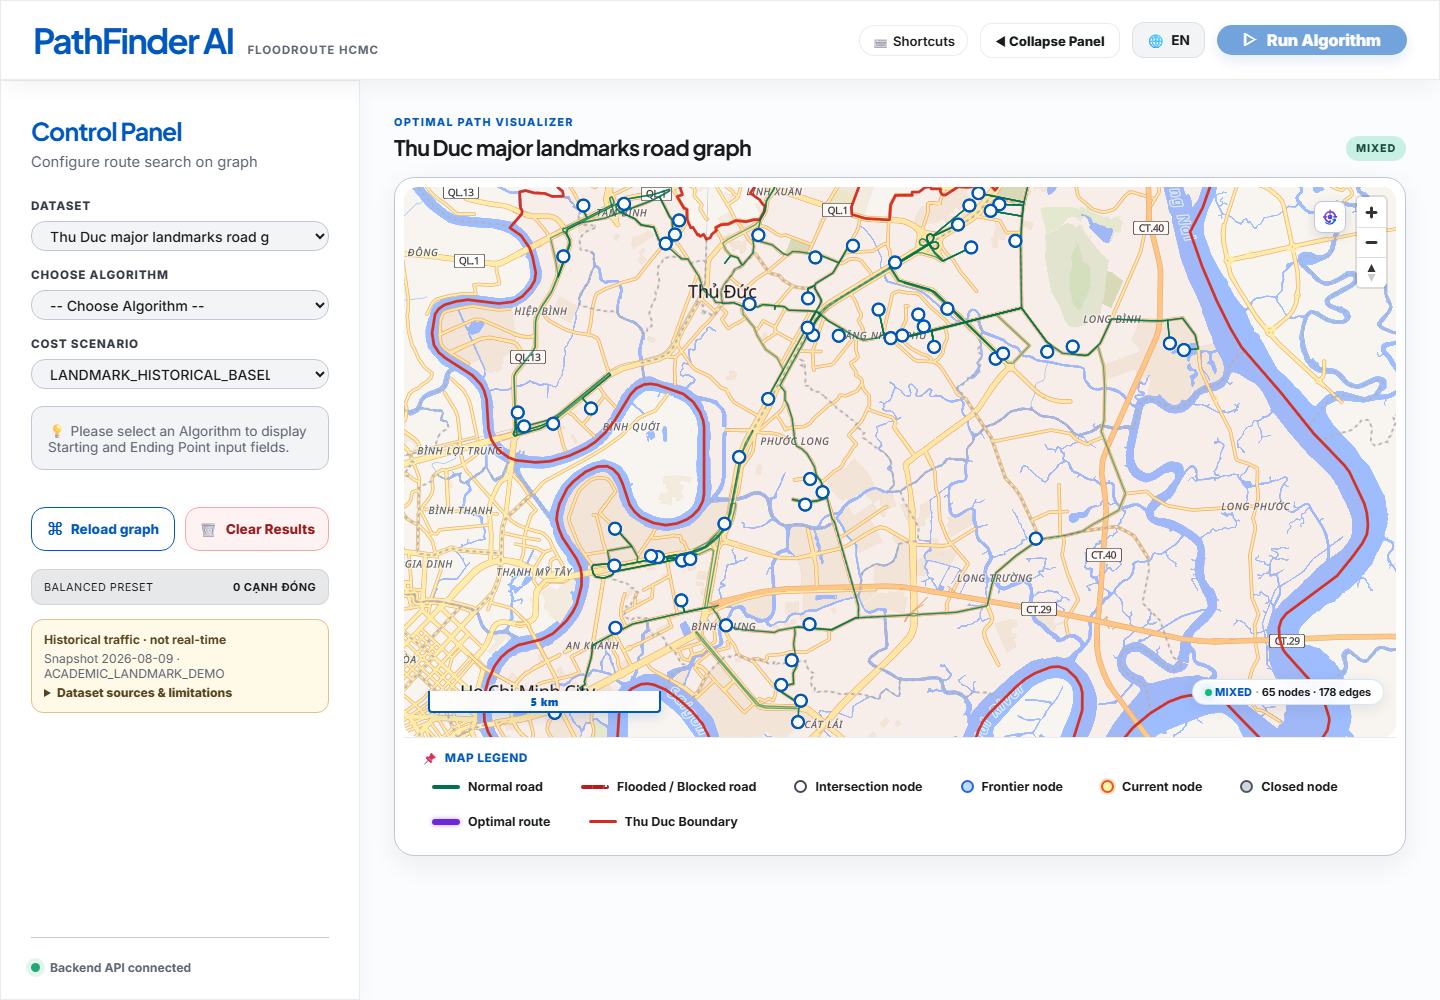
\includegraphics[width=\linewidth,height=.46\textheight,keepaspectratio]{gui-overview.png}\\
  {\scriptsize\textcolor{muted}{Landmark map và trạng thái các edge.}}
\end{column}
\end{columns}
\end{frame}

\begin{frame}{Mô hình graph}
\begin{center}
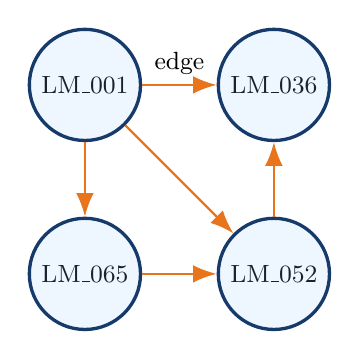
\begin{tikzpicture}[node distance=2.4cm, every node/.style={font=\small},
  n/.style={circle,draw=blue,very thick,fill=softblue,text=ink,minimum size=1cm},
  e/.style={-{Latex[length=3mm]},thick,draw=gold}]
  \node[n] (a) {LM\_001};
  \node[n,right of=a] (b) {LM\_036};
  \node[n,below of=b] (c) {LM\_052};
  \node[n,below of=a] (d) {LM\_065};
  \draw[e] (a) -- node[above]{edge} (b);
  \draw[e] (a) -- (c);
  \draw[e] (a) -- (d);
  \draw[e] (d) -- (c);
  \draw[e] (c) -- (b);
\end{tikzpicture}
\end{center}
\begin{itemize}
  \item Node: landmark và tọa độ địa lý.
  \item Edge: hướng đi, khoảng cách, thời gian, traffic, flood và trạng thái đóng.
  \item Graph không bị mutate trong quá trình tìm kiếm; tie-break deterministic.
\end{itemize}
\end{frame}

\begin{frame}{Pipeline dữ liệu}
\begin{columns}[c]
\column{.24\textwidth}\centering\pill{blue}{RAW}\\ snapshot
\column{.24\textwidth}\centering\pill{gold}{INTERIM}\\ lọc vùng
\column{.24\textwidth}\centering\pill{green}{PROCESSED}\\ release
\column{.24\textwidth}\centering\pill{purple}{SUBMISSION}\\ bundle
\end{columns}
\vfill
\begin{block}{Nguyên tắc dữ liệu}
Raw data bất biến; release có manifest, validation report và SHA-256 checksum.
\end{block}
\end{frame}

\begin{frame}{Các trường dữ liệu quan trọng}
\begin{tabularx}{\textwidth}{l X l}
\toprule
Trường & Ý nghĩa & Nhãn\\
\midrule
\texttt{distance\_m} & Chiều dài vật lý của aggregate edge & DERIVED\\
\texttt{free\_flow\_time\_min} & Thời gian khi đường thông & SOURCE/DERIVED\\
\texttt{traffic\_penalty\_min} & Độ trễ do kẹt xe & SIMULATED\\
\texttt{flood\_risk\_0\_1} & Mức rủi ro ngập chuẩn hóa & ASSUMPTION\\
\texttt{is\_closed} & Edge có bị loại khỏi tìm kiếm không & SCENARIO\\
\bottomrule
\end{tabularx}
\vspace{5mm}
\begin{block}{Free-flow time}
\centering $t(e)=\dfrac{distance\_km(e)}{speed\_kmh(e)}\times 60$; connector landmark dùng giả định 20 km/h.
\end{block}
\end{frame}

\begin{frame}{Hàm chi phí 4 thành phần}
\begin{equation*}
C_s(e)=w_dD(e)+w_tT_{ff}(e)+w_cP_{traffic,s}(e)+w_fR_{flood,s}(e)
\end{equation*}
\begin{columns}[T]
\column{.24\textwidth}\centering\key{Distance}\\Khoảng cách
\column{.24\textwidth}\centering\key{Free-flow}\\Thời gian cơ sở
\column{.24\textwidth}\centering\key{Congestion}\\Độ trễ kẹt xe
\column{.24\textwidth}\centering\key{Flood risk}\\Rủi ro ngập
\end{columns}
\vfill
\begin{alertblock}{Closure}
Edge đóng là hard constraint: không được xuất hiện trong neighbors hoặc route, bất kể weight.
\end{alertblock}
\end{frame}

\begin{frame}{Cost profiles}
\begin{center}
\begin{tabular}{lcccc}
\toprule
Profile & Distance & Time & Congestion & Flood\\
\midrule
BALANCED & 0.25 & 0.30 & 0.20 & 0.25\\
PEAK\_TRAFFIC & 0.15 & 0.25 & 0.45 & 0.15\\
RAIN\_SAFE & 0.10 & 0.25 & 0.15 & 0.50\\
\bottomrule
\end{tabular}
\end{center}
\vfill
\smallnote{Các weight là hệ số ưu tiên của prototype, không phải phần trăm đóng góp vì các thành phần khác đơn vị và scale.}
\end{frame}

\begin{frame}{Bốn scenario trên frontend}
\begin{tabularx}{\textwidth}{l X}
\toprule
Scenario & Cách hoạt động\\
\midrule
NORMAL & Không có cản trở; baseline cho tuyến ngắn nhất khả thi.\\
CONGESTION & 57/283 edge có traffic penalty, xấp xỉ 20\%.\\
FLOOD & 57/283 edge có flood risk, xấp xỉ 20\%.\\
RANDOM & Mỗi lần nhấn sinh seed mới và chọn đồng thời closure, flood, congestion.\\
\bottomrule
\end{tabularx}
\vfill
\centering\pill{green}{SIMULATED / ASSUMPTION -- không phải dữ liệu real-time}
\end{frame}

\begin{frame}{Random scenario: cả kẹt và ngập}
\begin{center}
\begin{tikzpicture}[node distance=2.2cm, every node/.style={font=\small},
  b/.style={rounded corners,draw=blue,fill=softblue,text=ink,minimum width=2.7cm,minimum height=0.9cm},
  a/.style={-{Latex[length=3mm]},very thick,draw=gold}]
  \node[b] (seed) {Seed mới};
  \node[b,below left=1cm and 0.8cm of seed] (close) {1 CLOSED};
  \node[b,below=1cm of seed] (flood) {3 FLOODED};
  \node[b,below right=1cm and 0.8cm of seed] (cong) {3 CONGESTED};
  \draw[a] (seed)--(close); \draw[a] (seed)--(flood); \draw[a] (seed)--(cong);
\end{tikzpicture}
\end{center}
\vfill
\centering Mỗi lần regenerate, tập edge và trạng thái trên map được thay mới.
\end{frame}

\begin{frame}{Hard closure và detour}
\begin{itemize}
  \item \texttt{closed\_edge\_ids} và \texttt{edge\_overrides.is\_closed} đều được Graph contract xử lý thống nhất.
  \item Tất cả thuật toán chỉ nhìn thấy edge mở trong `neighbors()`.
  \item Nếu không còn tuyến, API trả \texttt{NO\_ROUTE}.
  \item Closure áp dụng theo landmark edge; không lan sang aggregate edge khác chỉ vì hình học chồng lấn.
\end{itemize}
\begin{alertblock}{Kết quả mong muốn}
Không thuật toán nào được phép đi xuyên qua cạnh đã đóng.
\end{alertblock}
\end{frame}

\begin{frame}{Sáu thuật toán tìm kiếm}
\begin{tabular}{lll}
\toprule
Nhóm & Thuật toán & Đặc điểm\\
\midrule
Không trọng số & BFS & Ít số chặng nhất; không tối ưu cost tổng quát\\
Không trọng số & DFS & Khám phá sâu; không bảo đảm tối ưu\\
Có trọng số & UCS/Dijkstra & Tối ưu composite cost\\
Có trọng số & A* & UCS + heuristic lower-bound\\
Heuristic & Greedy Best-First & Nhanh; không bảo đảm tối ưu\\
Mở rộng & Bidirectional & Tìm từ hai hướng; cần điều kiện dừng phù hợp\\
\bottomrule
\end{tabular}
\end{frame}

\begin{frame}{BFS và DFS}
\begin{columns}[T]
\column{.48\textwidth}
\begin{block}{BFS}
\begin{itemize}
  \item Queue FIFO.
  \item Mở rộng theo độ sâu.
  \item Tối ưu số hop khi mọi edge có cùng cost.
\end{itemize}
\end{block}
\column{.48\textwidth}
\begin{block}{DFS}
\begin{itemize}
  \item Stack LIFO.
  \item Đi sâu theo một nhánh trước.
  \item Dùng \texttt{expanded} để tránh chu trình.
\end{itemize}
\end{block}
\end{columns}
\vfill\centering\smallnote{Cả hai vẫn tuân thủ Graph contract và hard closure.}
\end{frame}

\begin{frame}{UCS / Dijkstra}
\begin{block}{Nguyên lý}
Mở rộng node có $g(n)$ nhỏ nhất bằng min-heap.
\end{block}
\begin{equation*}
g(v)=\min_{u\to v}\{g(u)+C_s(u,v)\}
\end{equation*}
\begin{itemize}
  \item Chi phí cạnh không âm $\Rightarrow$ UCS tìm được $C^*$ nhỏ nhất.
  \item Được dùng làm chuẩn đối chiếu tính đúng đắn của A*.
  \item Không dùng heuristic nên thường mở rộng nhiều node hơn A*.
\end{itemize}
\end{frame}

\begin{frame}{A* Search}
\begin{equation*}
f(n)=g(n)+h_s(n)
\end{equation*}
\begin{itemize}
  \item $g(n)$: cost đã tích lũy từ start.
  \item $h_s(n)$: lower bound từ node hiện tại đến goal.
  \item Scenario được freeze trong một lần search.
  \item A* trả route tối ưu theo composite cost khi heuristic admissible và consistent.
\end{itemize}
\end{frame}

\begin{frame}{Heuristic scenario-aware}
\begin{equation*}
\rho_s=\min_{e\;open}\frac{C_s(e)}{D_{geo}(e)},
\qquad h_s(n)=\rho_sD_{geo}(n,goal)
\end{equation*}
\begin{itemize}
  \item $C_s(e)$ đã bao gồm distance, time, congestion và flood risk.
  \item Edge đóng và cạnh có mẫu địa lý gần 0 không tham gia tính $\rho_s$.
  \item Heuristic không dư dữ kiện; nó là lower-bound cho đúng cost hiện tại.
\end{itemize}
\end{frame}

\begin{frame}{Bảo đảm đúng đắn}
\begin{block}{Admissibility}
$h_s(n)$ không vượt quá cost thật của bất kỳ đường đi nào từ $n$ đến goal.
\end{block}
\begin{block}{Consistency}
$h_s(u)\le C_s(u,v)+h_s(v)$ với mọi edge mở.
\end{block}
\begin{alertblock}{Kết luận}
UCS và A* tối ưu composite cost; route ngắn nhất được ưu tiên thông qua cost cơ sở và cách diễn giải kết quả.
\end{alertblock}
\end{frame}

\begin{frame}{Kiến trúc hệ thống}
\begin{center}
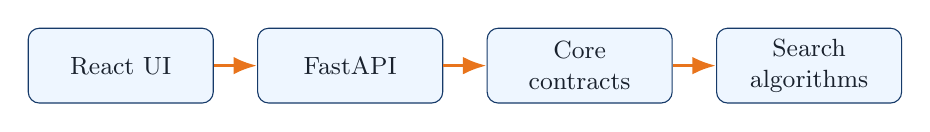
\begin{tikzpicture}[node distance=.55cm, every node/.style={font=\small},
  b/.style={rounded corners,draw=blue,fill=softblue,text=ink,minimum width=2.35cm,minimum height=.95cm,align=center},
  a/.style={-{Latex[length=3mm]},very thick,draw=gold}]
  \node[b] (ui) {React UI};
  \node[b,right=of ui] (api) {FastAPI};
  \node[b,right=of api] (core) {Core\\contracts};
  \node[b,right=of core] (alg) {Search\\algorithms};
  \draw[a] (ui.east) -- (api.west);
  \draw[a] (api.east) -- (core.west);
  \draw[a] (core.east) -- (alg.west);
\end{tikzpicture}
\end{center}
\vfill
\centering Graph và ScenarioCostEngine độc lập với FastAPI; thuật toán không mutate graph.
\end{frame}

\begin{frame}{Luồng chạy trên frontend}
\begin{enumerate}
  \item Chọn start, goal, algorithm và scenario.
  \item Gọi API search với graph/scenario hiện tại.
  \item Hiển thị route chính, trace frontier/current/closed và metrics.
  \item Nếu scenario có cản trở, gọi endpoint alternatives cùng algorithm.
  \item Người dùng chọn route để map chuyển highlight sang tuyến tương ứng.
\end{enumerate}
\end{frame}

\begin{frame}{Minh họa giao diện: bản đồ và route}
\begin{columns}[T]
\column{.49\textwidth}
\centering
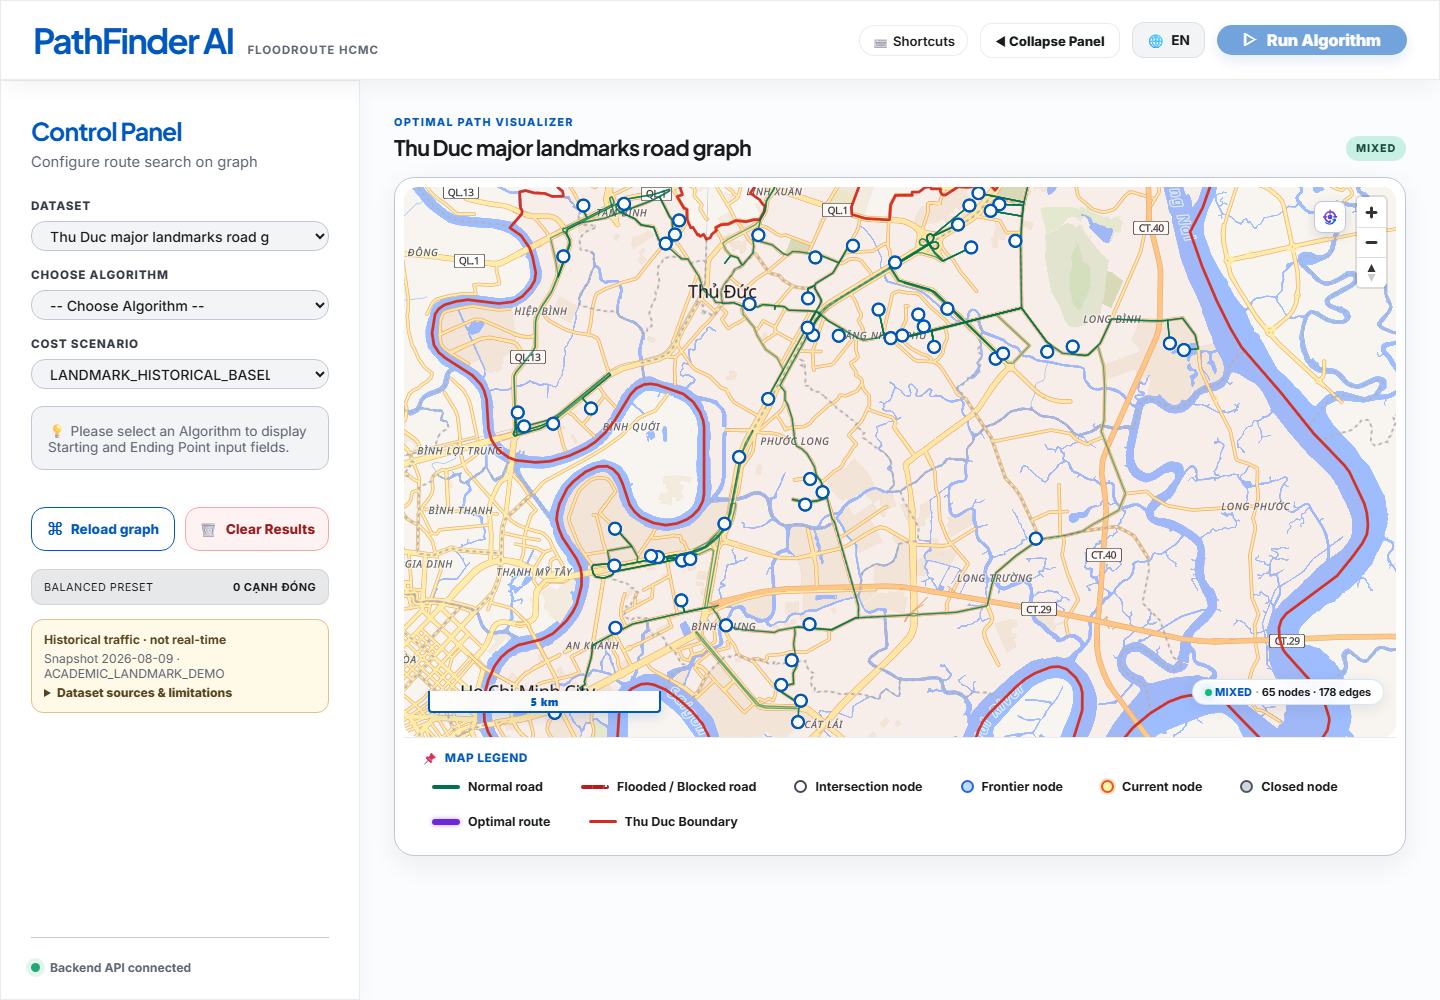
\includegraphics[width=\linewidth,height=.56\textheight,keepaspectratio]{gui-overview.png}\\
{\scriptsize\textcolor{muted}{Bản đồ landmark và trạng thái edge.}}
\column{.49\textwidth}
\centering
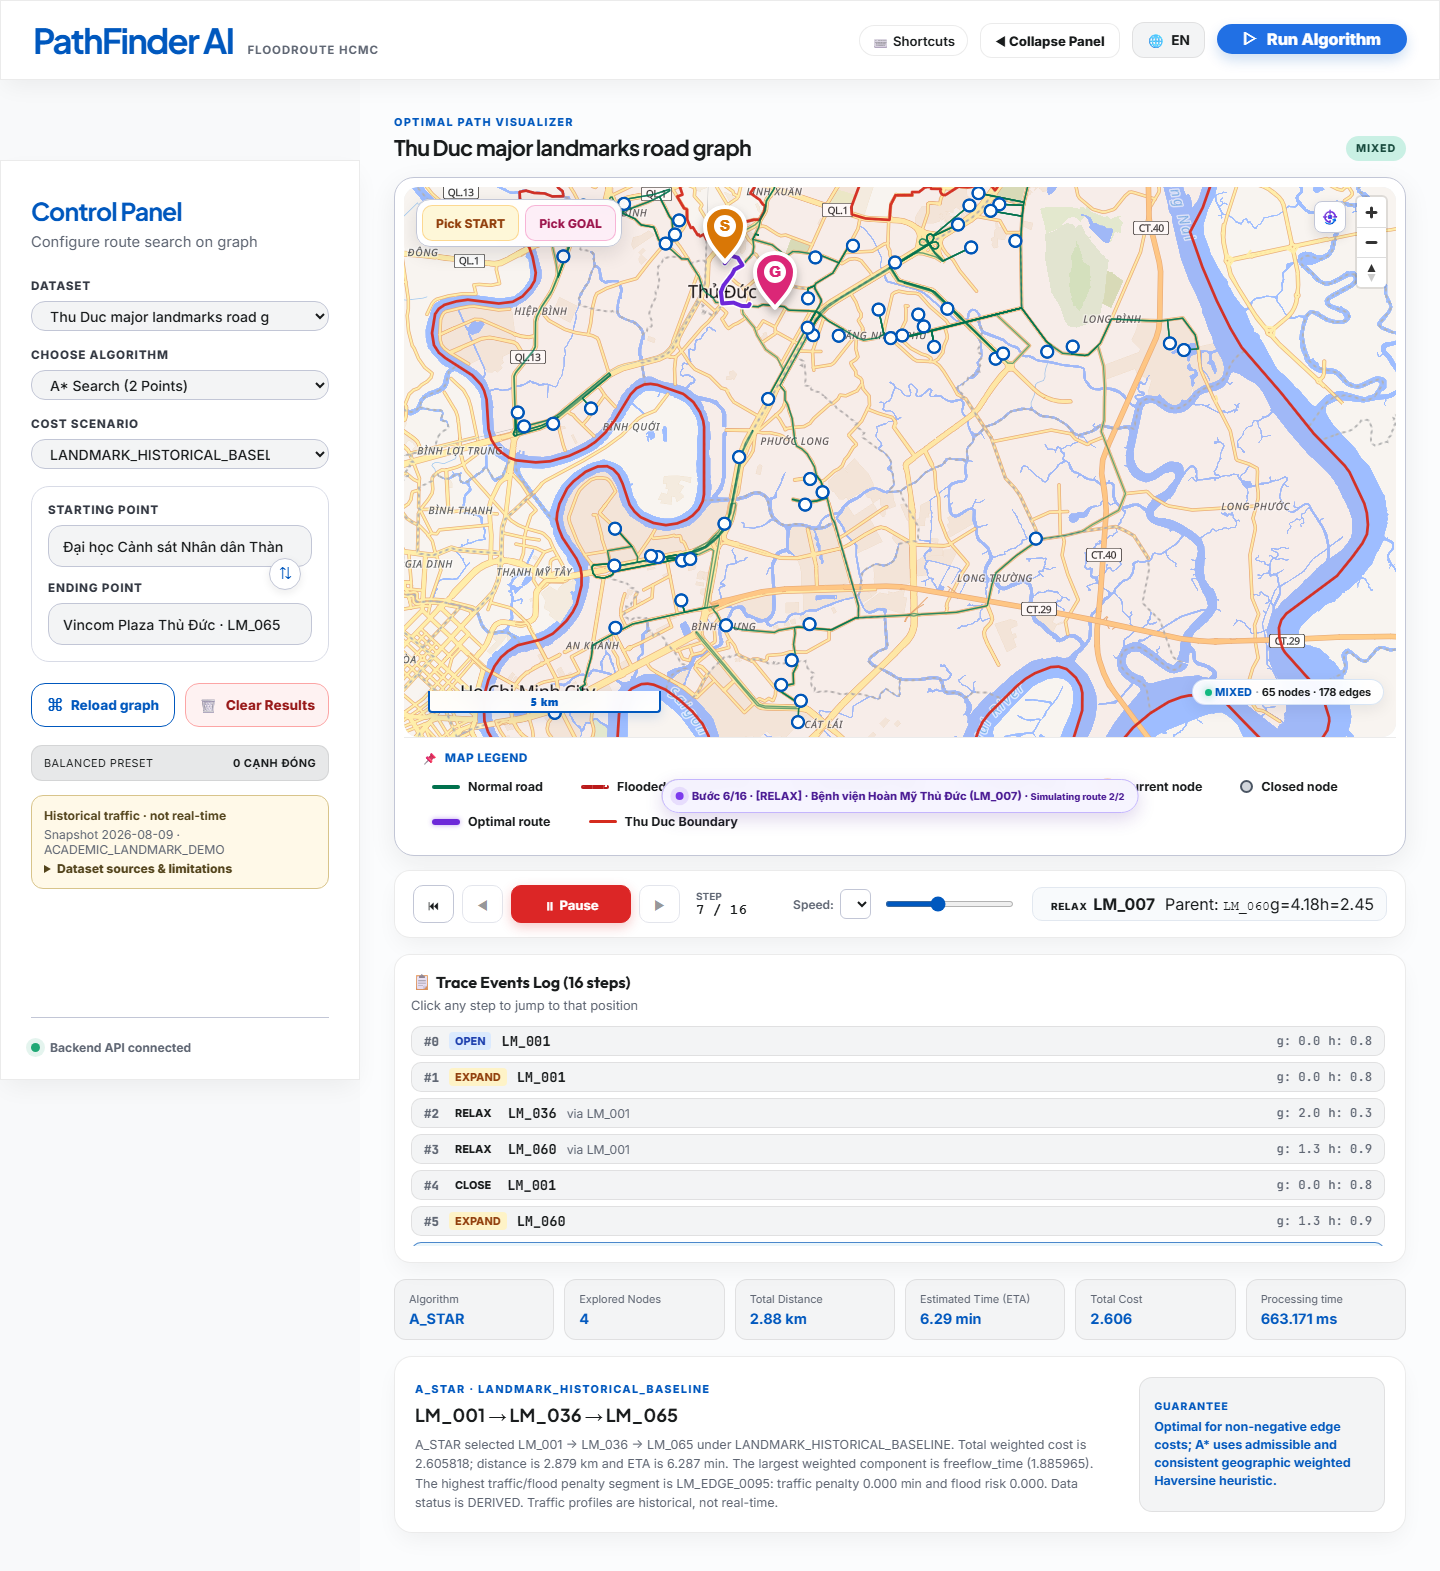
\includegraphics[width=\linewidth,height=.56\textheight,keepaspectratio]{gui-astar-route.png}\\
{\scriptsize\textcolor{muted}{Route và trace của A*.}}
\end{columns}
\end{frame}

\begin{frame}{Minh họa giao diện: so sánh và tour}
\begin{columns}[T]
\column{.49\textwidth}
\centering
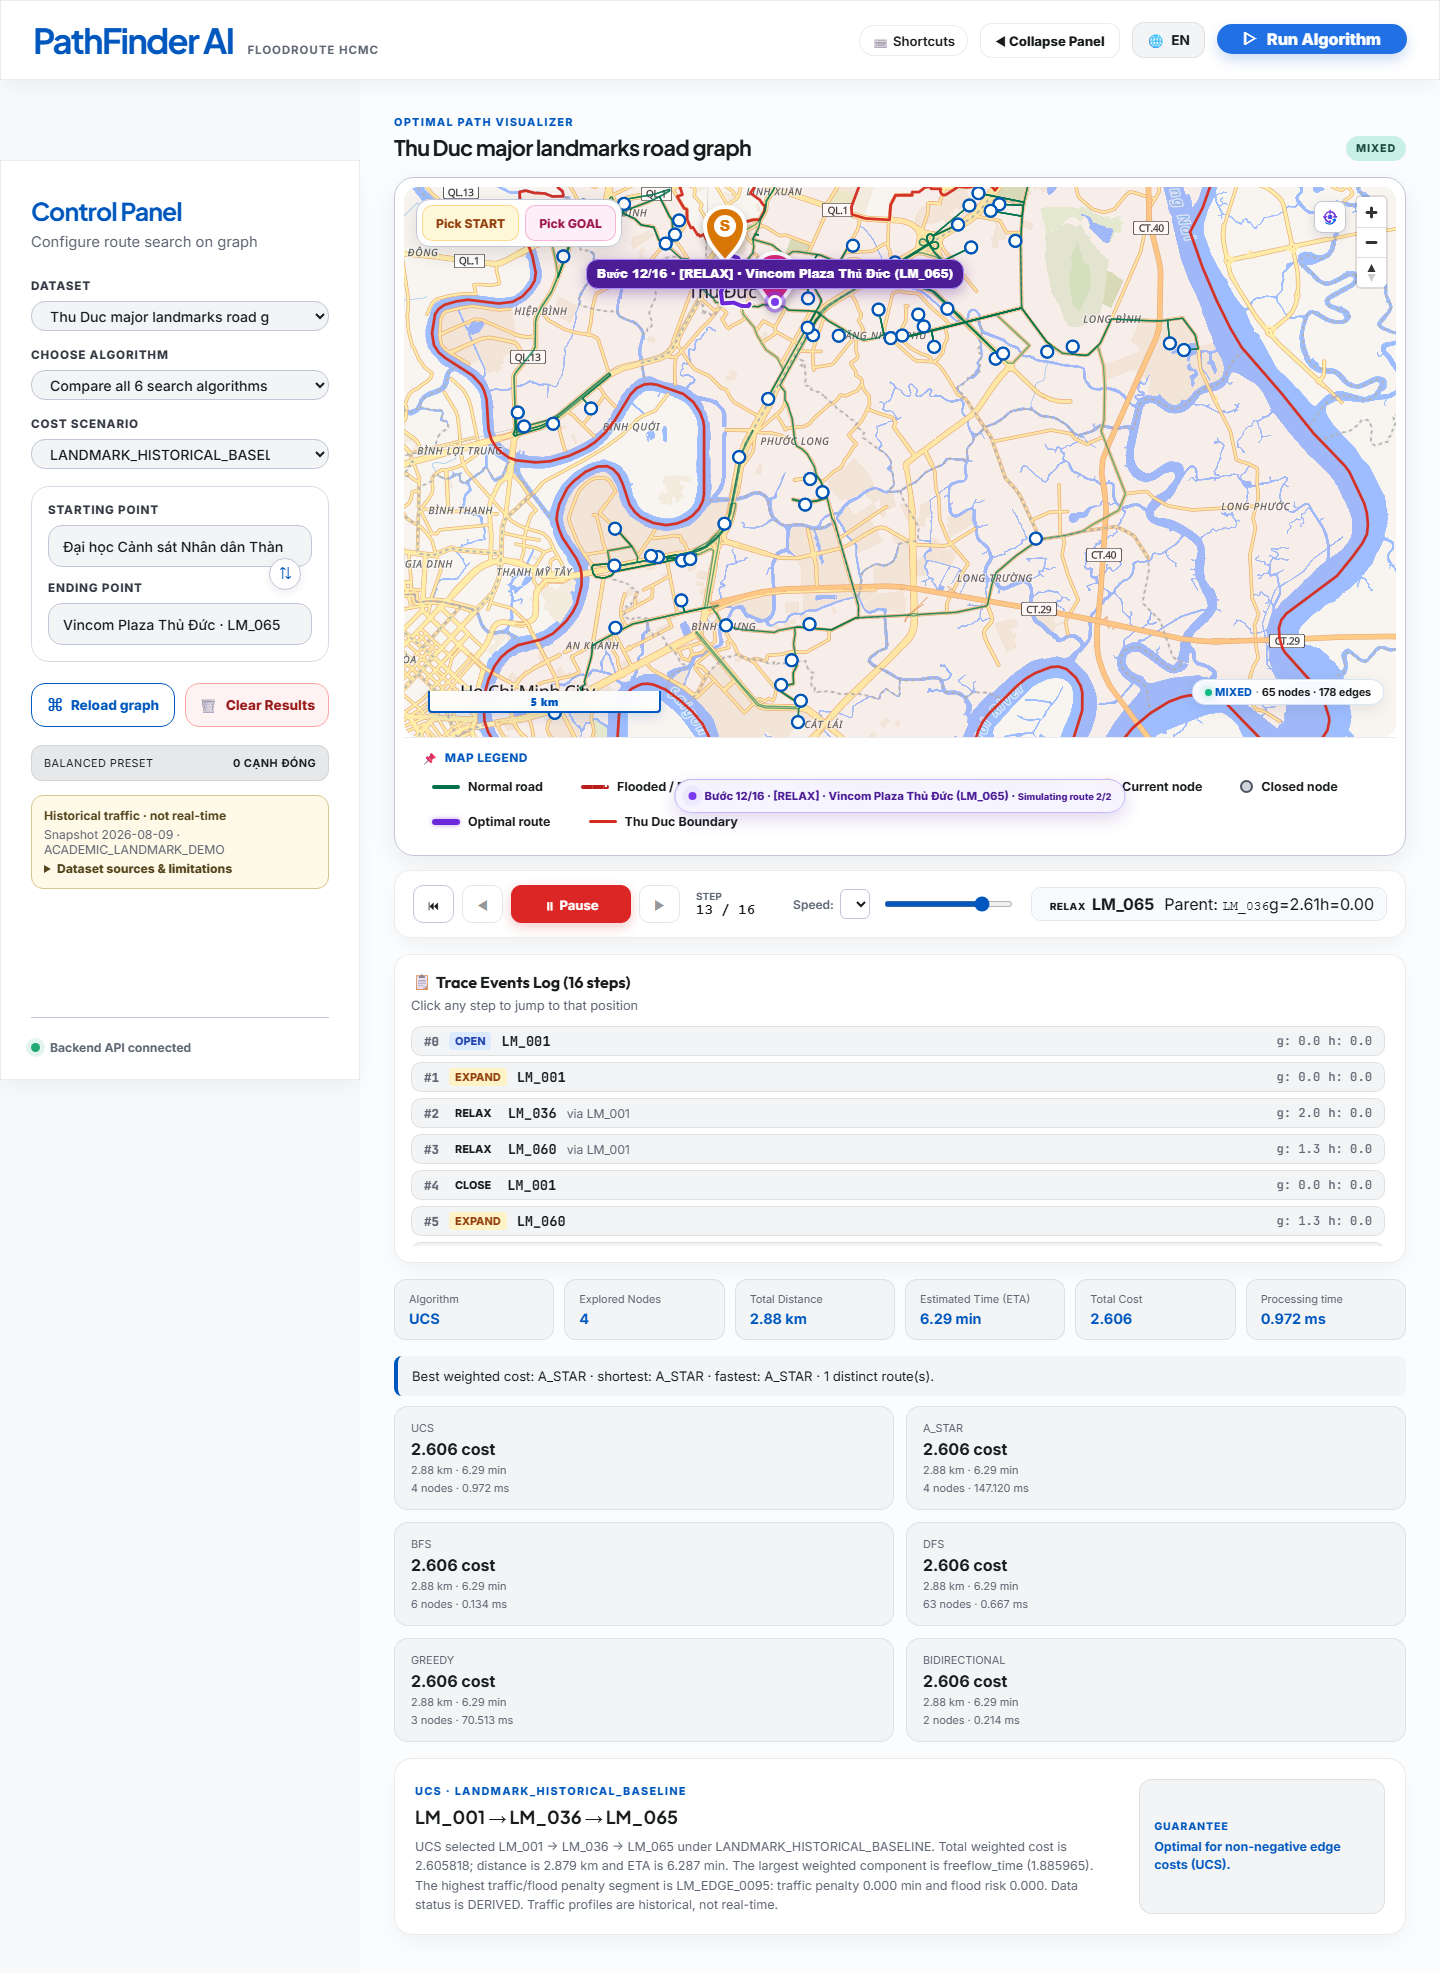
\includegraphics[width=\linewidth,height=.56\textheight,keepaspectratio]{gui-compare-algorithms.png}\\
{\scriptsize\textcolor{muted}{So sánh kết quả các thuật toán.}}
\column{.49\textwidth}
\centering
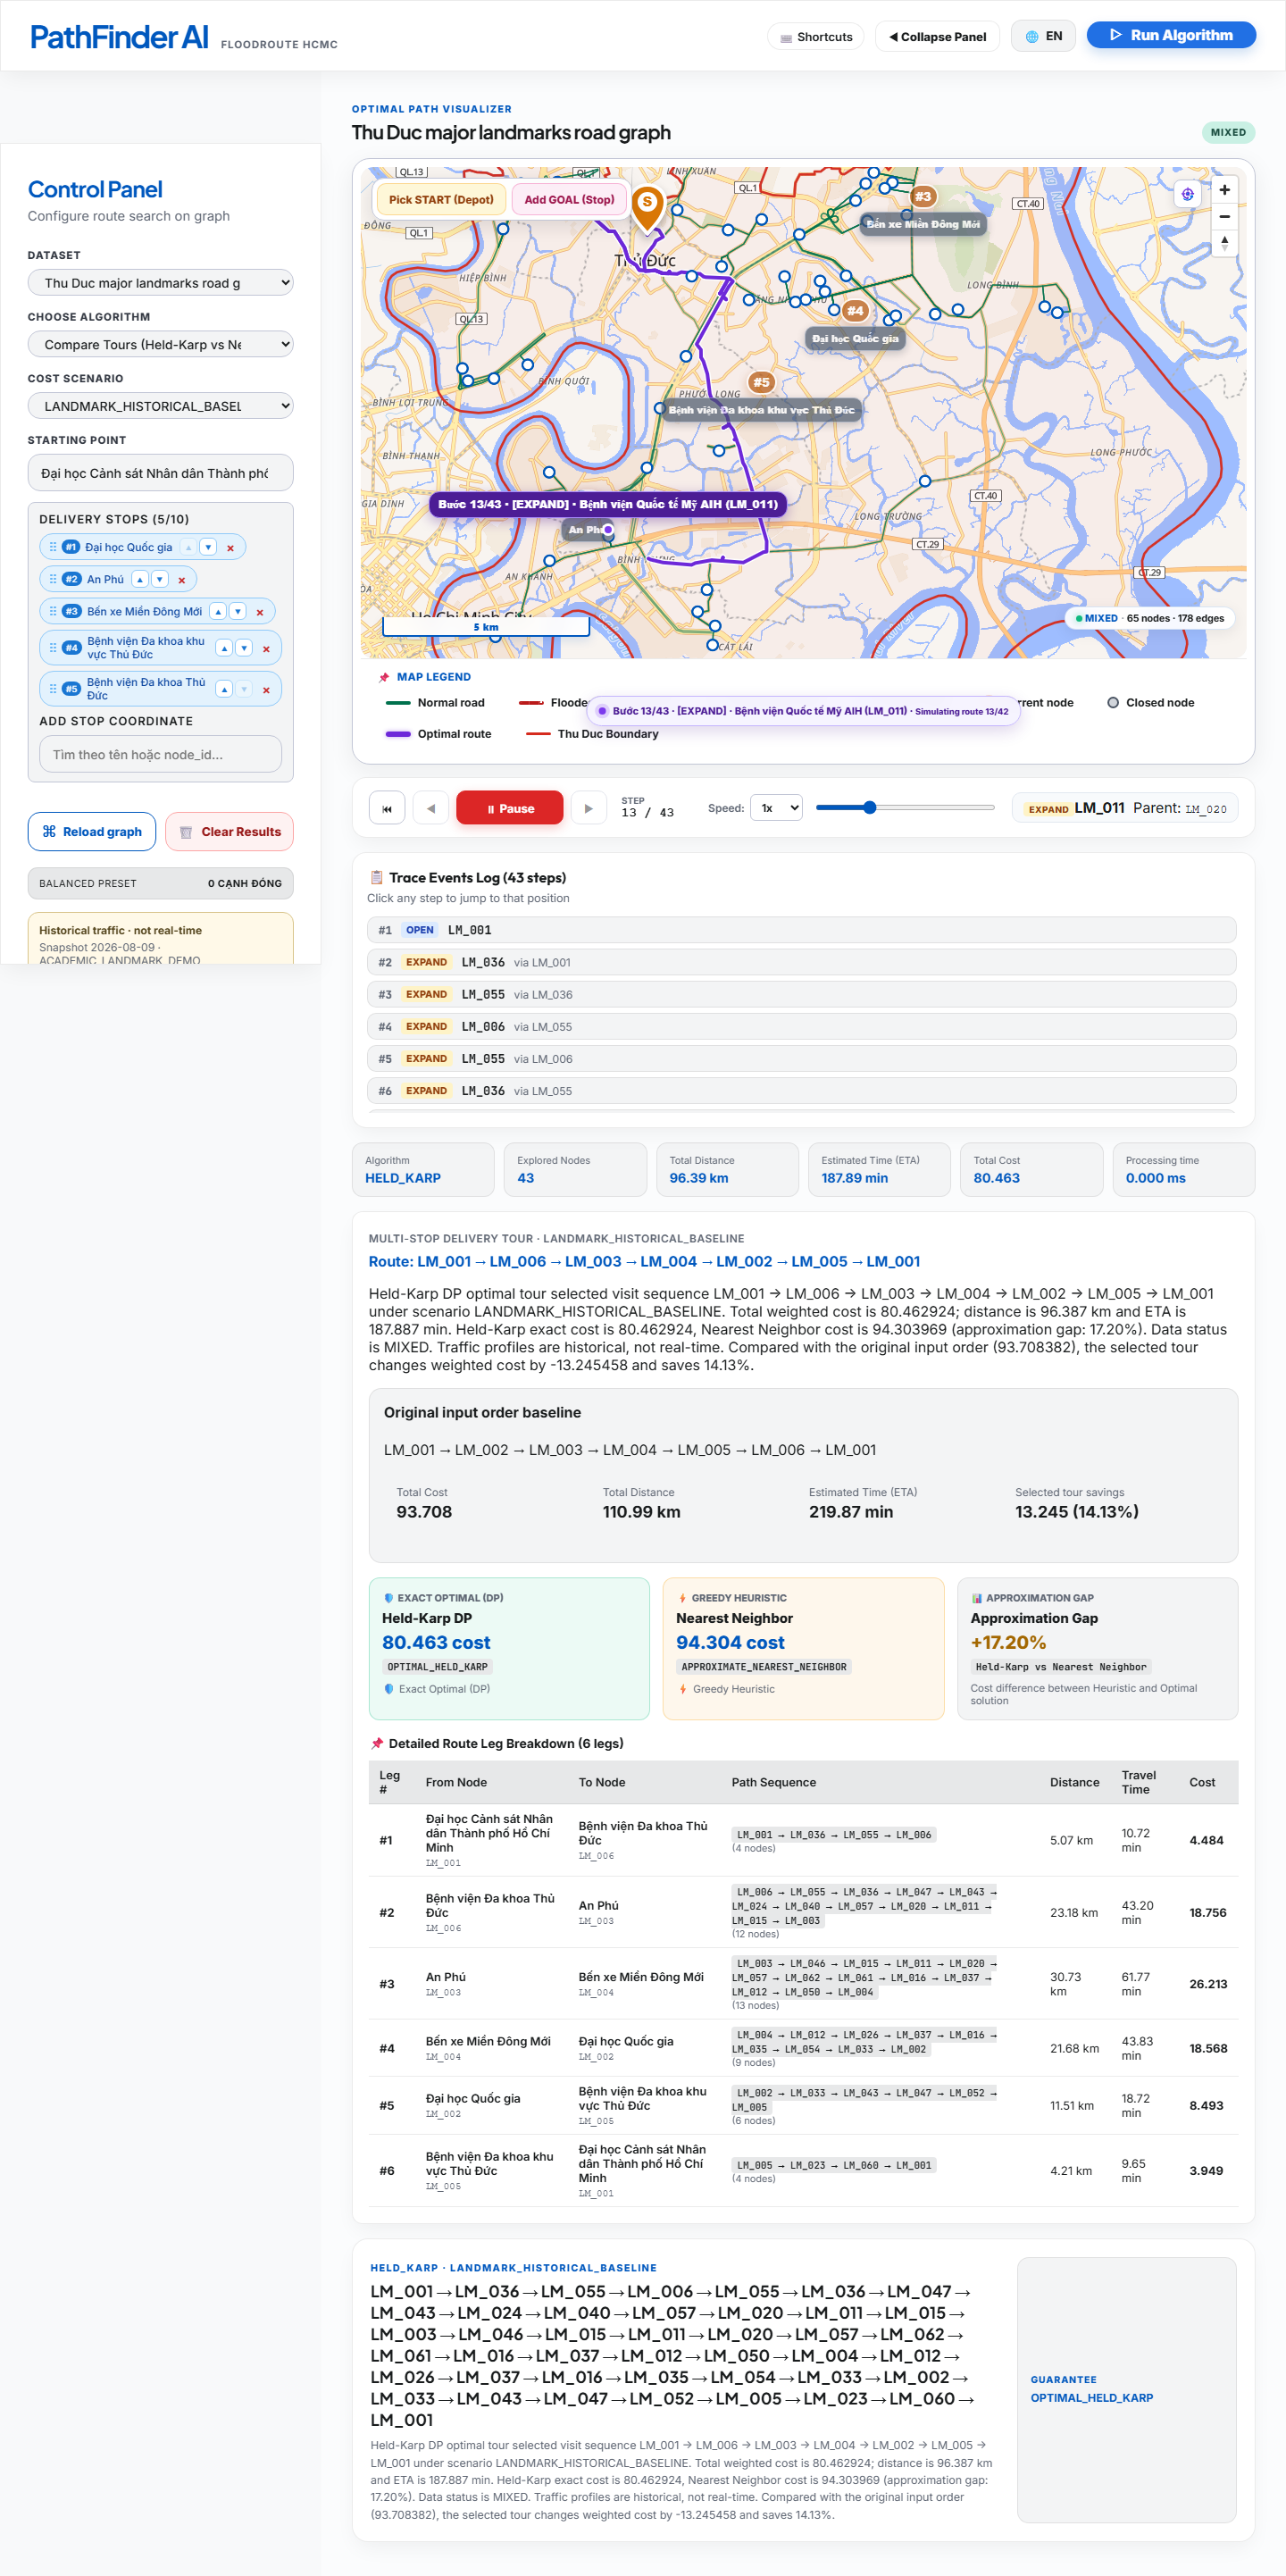
\includegraphics[width=\linewidth,height=.56\textheight,keepaspectratio]{gui-tour-optimization.png}\\
{\scriptsize\textcolor{muted}{Tối ưu tour nhiều điểm giao hàng.}}
\end{columns}
\end{frame}

\begin{frame}{Các tuyến thay thế}
\begin{itemize}
  \item Dùng chính thuật toán người dùng đã chọn, không trộn kết quả của thuật toán khác.
  \item Tạm loại một edge trên route chính để tìm detour mới.
  \item Trả tối đa hai route thay thế khác nhau.
  \item Mỗi thẻ hiển thị distance, ETA và total cost.
  \item Thẻ có cost thấp nhất được đánh dấu tối ưu trong scenario hiện tại.
\end{itemize}
\end{frame}

\begin{frame}{Trực quan hóa bản đồ}
\begin{center}
\small
\renewcommand{\arraystretch}{1.18}
\begin{tabular}{lll}
\toprule
Màu & Trạng thái & Ý nghĩa\\
\midrule
\textcolor{green}{Xanh lá} & Open & Đường lưu thông\\
\textcolor{gold}{Vàng} & Congested & Đường bị kẹt\\
\textcolor{blue}{Xanh dương} & Flooded & Đường bị ngập\\
\textcolor{red}{Đỏ nét đứt} & Closed & Đường bị đóng\\
\textcolor{purple}{Tím} & Selected & Tuyến đang được chọn\\
\bottomrule
\end{tabular}
\end{center}
\vfill
\centering\smallnote{Legend song ngữ Việt/Anh được đặt trực tiếp trên map.}
\end{frame}

\begin{frame}{Bài toán nhiều điểm giao hàng}
\begin{block}{Pairwise matrix}
Tính cost và thời gian ngắn nhất giữa depot và các điểm giao.
\end{block}
\begin{columns}[T]
\column{.48\textwidth}
\begin{block}{Held--Karp DP}
Nghiệm chính xác cho số stop nhỏ. Độ phức tạp tăng theo cấp số mũ.
\end{block}
\column{.48\textwidth}
\begin{block}{Nearest Neighbor}
Heuristic nhanh: mỗi bước chọn điểm chưa thăm có pairwise cost nhỏ nhất.
\end{block}
\end{columns}
\end{frame}

\begin{frame}{Thiết kế kiểm thử}
\begin{itemize}
  \item Data validator: kiểm tra manifest, checksum, schema và số node/edge.
  \item Backend tests: contract, cost, closure, random scenario, search.
  \item Frontend tests: scenario selector, map status, route selection.
  \item A*/UCS lower-bound: so sánh cost và số node khám phá.
  \item Build LaTeX: biên dịch hai lượt và render kiểm tra bố cục.
\end{itemize}
\end{frame}

\begin{frame}{Kết quả và cách diễn giải}
\begin{block}{Điều được chứng minh}
Trong các case kiểm thử, A* trả cùng composite cost với UCS khi dùng cùng graph và scenario.
\end{block}
\begin{block}{Điều được quan sát}
Khi kẹt/ngập làm tăng cost hoặc closure loại cạnh, route có thể đổi sang detour dài hơn nhưng khả thi hơn.
\end{block}
\begin{alertblock}{Cách gọi chính xác}
“Tuyến tối ưu theo composite cost”, không khẳng định là khoảng cách ngắn nhất tuyệt đối trong mọi scenario.
\end{alertblock}
\end{frame}

\begin{frame}{Giới hạn dữ liệu và mô hình}
\begin{itemize}
  \item Traffic là historical snapshot, chưa phải live telemetry.
  \item Flood là danh mục/risk giả lập, chưa có hydraulic dynamic model.
  \item Weight là hệ số prototype; các đơn vị chưa được chuẩn hóa thành tiền hoặc thời gian duy nhất.
  \item Aggregate edge giữ topology landmark, không phải toàn bộ mạng road segment.
  \item Random scenario có seed mới mỗi lần nên cần lưu seed nếu muốn tái lập chính xác.
\end{itemize}
\end{frame}

\begin{frame}{Các trường hợp có thể làm kết quả sai}
\footnotesize
\begin{itemize}
  \item \textbf{Snap sai start/goal}: địa chỉ giữa hai landmark bị gán vào node gần nhất nên route bắt đầu/kết thúc lệch vị trí.
  \item \textbf{Sai hướng cạnh}: graph chỉ có LM\_001 $\rightarrow$ LM\_036; tìm chiều ngược có thể trả \texttt{NO\_ROUTE} dù người dùng nghĩ đường hai chiều.
  \item \textbf{Closure không theo hình học}: đóng một landmark edge không tự đóng aggregate edge khác đang chồng lấn cùng đoạn đường.
  \item \textbf{Scenario bị stale}: RANDOM đổi seed sau khi search làm màu edge, cost và route không còn cùng một trạng thái.
  \item \textbf{Cost khác mục tiêu}: A*/UCS tối ưu composite cost, không đảm bảo ngắn nhất theo mét nếu flood/congestion weight cao.
  \item \textbf{Graph thưa hoặc dữ liệu lỗi}: closure có thể dẫn đến \texttt{NO\_ROUTE}; tọa độ đảo lat/lon hoặc polyline lỗi cũng làm khoảng cách sai.
\end{itemize}
\begin{alertblock}{Cách diễn giải}
Kết quả có thể đúng theo graph và contract, nhưng vẫn không đúng với thực tế nếu dữ liệu, scenario hoặc cost model không đại diện đủ.
\end{alertblock}
\end{frame}

\begin{frame}{Định hướng phát triển}
\begin{enumerate}
  \item Kết nối traffic và flood real-time.
  \item Hiệu chỉnh tốc độ theo dữ liệu đo thực tế.
  \item Tách rõ chế độ tối ưu khoảng cách và composite cost.
  \item Hỗ trợ custom weights có validation.
  \item Mở rộng nhiều xe, capacity và time windows.
\end{enumerate}
\end{frame}

\begin{frame}{Kết luận}
\begin{itemize}
  \item FloodRoute mô hình hóa bài toán giao thông bằng graph 65 node/283 directed edge.
  \item Mục tiêu chính là ưu tiên tuyến đường ngắn nhất khả thi.
  \item Kẹt xe, ngập nước và closure được thể hiện minh bạch trên map và trong cost.
  \item UCS/A* cung cấp nghiệm tối ưu theo composite cost; các thuật toán khác giúp so sánh hành vi tìm kiếm.
  \item Frontend cho phép quan sát route, trace, scenario và tuyến thay thế trong cùng một giao diện.
\end{itemize}
\vfill
\centering{\Large\color{blue}\textbf{Cảm ơn thầy cô và các bạn đã lắng nghe!}}
\end{frame}

\end{document}
